\documentclass[11pt]{article}
%Gummi|063|=)

\usepackage{ntheorem}
\usepackage{amssymb}
\usepackage[T1]{fontenc}
\usepackage[utf8]{inputenc}
\usepackage{amsmath}
\usepackage{graphicx}
\usepackage{float}

\newcommand{\RN}[1]{\uppercase\expandafter{\romannumeral #1\relax}}
\renewcommand\thesubsection{\thesection\alph{subsection})}



\title{\textbf{Econometrics Take Home Exam 2}}
\author{Johannes Degn 01/848553}
\date{18.01.2012}

\theoremstyle{break}

\begin{document}
\maketitle


\section{Problem}
Random Seed for the whole problem: "rndseed 1;"

\subsection{}
Heteroskedasticity means that the error term of each observation has a potentially different variance depending on i. I.e. the conditional variance $V(e_i|X_i)$ differs among groups of observations or for every observation. If we use the model $Y_i = \beta X_i + \varepsilon_i$ the variance of $\varepsilon_i$ carries an index $i$ to denote that it differs among observations. One simple example where this might occur is if $X_i$ denotes gender and $Y_i$ denotes income. For heteroscedasticity we might observe that the variance among the income of the male observations is different to the variance of the female observations. This might for example happen if there are more men with very high and very low incomes while female observations are clustered more around the mean of the whole population.

Heteroscedasticity can be an issue because the estimates for the variance of parameters which do not account for heteroscedasticity can become inconsistent and biased (the point estimates can still be consistent but no longer efficient). In the example of OLS, the parameter estimates will still be consistent but hypothesis tests might yield wrong results.

Figure \ref{heteroscedasticity} below shows a random example where $X_i \;{\buildrel d \over \rightarrow}\; U(-1, 1)$, $\varepsilon_i \;{\buildrel d \over \rightarrow}\; N(0, X_i^2)$, $\beta = 1$ and $Y = X_i\beta+\varepsilon_i$

\begin{figure}[H]
\centering
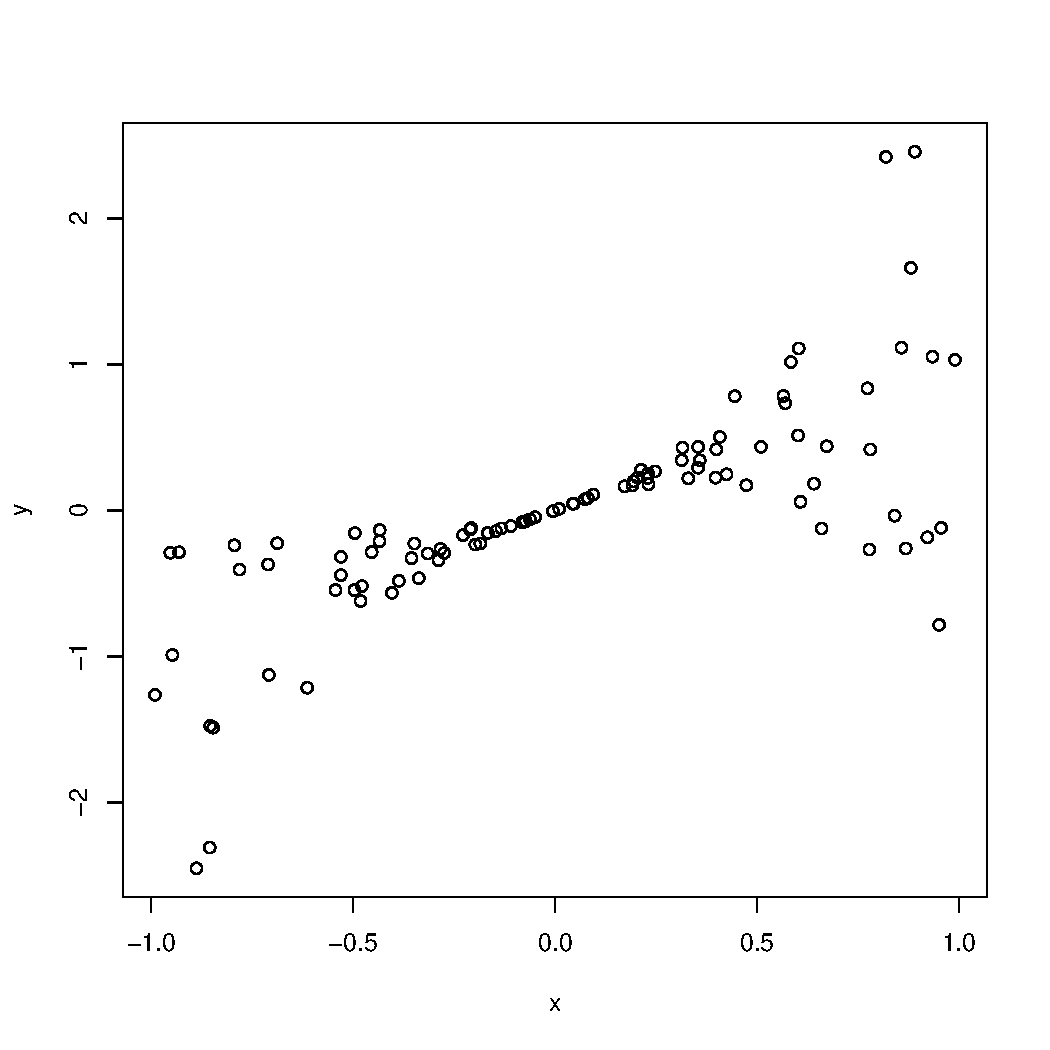
\includegraphics[height=100mm]{heteroscedasticity.pdf}
\caption{Heteroscedasticity}
\label{heteroscedasticity}
\end{figure}


\subsection{}
Let $A(X_i) = X_i\exp(-X_i)$ be the matrix of instruments and let $\rho(Z_i, \beta) = \varepsilon_i = (Y_i - X\beta)$. $\rho(Z_i, \beta)$ is a well defined conditional moment function for $\tilde{\beta}$ since $E(\rho(Z_i, \beta)| X_i) = E(\varepsilon_i | X_i) = 0$. Then $\psi(Z_i, \beta) = A(X_i)'\rho(z_i, \beta) = \exp(-X_i)X_i(Y_i-\beta X_i)$
\\
$\psi(Z_i, \beta) = \exp(-X_i)X_i(Y_i - \beta X_i)$ is a moment function that corresponds to $\tilde{\beta}$. $\psi(Z_i, \beta)$ is a well defined moment function because $E(\psi(Z_i, \beta)) = E(\exp(-X_i)X_i\varepsilon_i) = \underset{x}{E}(E(\exp(-X_i)X_i\varepsilon_i|X_i)) = \underset{x}{E}(\exp(-X_i)X_iE(\varepsilon_i|X_i)) = 0$. \\

Since we have $q=1$ moment function and $k=1$ parameter, we can simply replace the population moments with the sample moments in order to get a method of moments estimator: \\
$$E(\psi(Z_i, \beta)) = 0$$
$$E(\exp(-X_i)X_i(Y_i -X_i\beta)) = 0$$
$$\frac{1}{n}\displaystyle \sum_{i=1}^n(\exp(-X_i)X_i(Y_i -X_i\tilde{\beta})) = 0$$
$$\displaystyle \sum_{i=1}^n(\exp(-X_i)X_iY_i) = \displaystyle \sum_{i=1}^n(\exp(-X_i)X_i^2\tilde{\beta})$$
$$\tilde{\beta} = \frac{\sum_{i=1}^n(\exp(-X_i)X_iY_i)}{\sum_{i=1}^n(\exp(-X_i)X_i^2
)}$$


\subsection{}
From proposition 5.2.1 from the lecture notes it follows that: \\
$\sqrt{n}(\tilde{\beta}_n-\beta) \;{\buildrel d \over \rightarrow}\; N(0, E(\frac{\partial \psi(Z_i, \beta_0)}{\partial \beta'})^{-1})V_0 E(\frac{\partial \psi(Z_i, \beta_0)}{\partial \beta})^{-1})$ \\
and $\tilde{\beta} \;{\buildrel d \over \rightarrow}\; N(\beta_0, E(\frac{\partial \psi(Z_i, \beta_0)}{\partial \beta'})^{-1}\frac{V_0}{n} E(\frac{\partial \psi(Z_i, \beta_0)}{\partial \beta})^{-1})$. \\

In our case we have $V_0 = V(\psi(Z_i, \beta_0)) = E(\psi(Z_i, \beta)^2) = E(\exp(-2X_i)\varepsilon_i^2X_i^2) = E(\underset{x}{E}(\exp(-2X_i)\varepsilon_i^2X_i^2|X_i)) = E(\exp(-2X_i)X_i^2\underset{x}{E}(\varepsilon_i^2|X_i)) = E(\exp(-X_i)X_i^2)$ and $\frac{\partial \psi(Z_i, \beta_0)}{\partial \beta'} = -\exp(-X_i)X_i^2$. \\
Thus: \\
$V(\tilde{\beta}) = E(-\exp(-X_i)X_i^2)^{-1}\frac{E(\exp(-X_i)X_i^2)}{n}E(-\exp(-X_i)X_i^2)^{-1} = \frac{E(\exp(-X_i)X_i^2)^{-1}}{n}$. Replacing the population moment with the sample moment yields the given variance estimator: \\
$\hat{V}(\tilde{\beta}) = \frac{1}{n}\frac{1}{\frac{1}{n} \sum_{i=1}^n\exp(-X_i)X_i^2}$.

\subsection{}
I expect both estimators to be consistent which can be seen by taking the plim. Also, since both estimators are MM estimators, the results from the lecture regarding consistency should hold. \\
The precision of an estimator is inverse to the variance and equivalent to efficiency. $\hat{\beta}$ is the White variance estimator for OLS which we know to be inefficient for a model with heteroscedasticity. $\tilde{\beta}$ is an MM estimator for which we have: $E(\psi(Z_i, \beta)) = 0$. Since we have $\varepsilon_i = Y_i - \beta X_i \;{\buildrel d \over \rightarrow}\; N(0, \exp(X_i))$. The log likelihood function for $\varepsilon_i$ is $\ln L(Z_i, \beta) = -\frac{n}{2}\ln(2\pi) - \frac{1}{2}\displaystyle\sum_{i=1}^n X_i - \displaystyle \sum_{i=1}^n \frac{(Y_i - \beta X_i)^2}{2\exp(X_i)}$ and the score function for one observation is $S_i(\beta) = \exp(-X_i)X_i(Y_i-\beta X_i)$ with $E(S_i(\beta)) = 0$. This is equivalent to the moment function we used earlier. We can thus see the moment estimator derrived earlier as a maximum likelihood estimator which we know to be efficient as it reaches the Cramer-Rao lower bound if the information equality holds. \\
More intuitively we can see that $\tilde{\beta}$ is the weighted least squares estimator with weight matrix as the inverse of the variance of $\varepsilon_i$. Since this corrects for the heteroscedastic variance while $\hat{\beta}$ does not, I expect $\tilde{\beta}$ to be more efficient.

\subsection{}
See Gauss code

\subsection{}
For the simulation: see Gauss code. \\
From the results we see that that both $\hat{\beta}$ and $\tilde{\beta}$ are consistent and approach 1 (the true $\beta$) for large $R$ and $n$. As proposed, the values of $\hat{V}(\tilde{\beta})$ are smaller than the average $\hat{V}(\hat{\beta}))$ which can also be seen in figure \ref{estimated variances}. \\
The RELSE values for $\hat{\beta}$ and $\tilde{\beta}$ both approach $1$ as n and R increase which indicates that the variance estimators and the variance of the estimators are similar on average which hints at the variance and point estimators being consistent. \\
The lower variance estimates for $\hat{V}(\tilde{\beta})$ result in higher t-statistics which lead to higher rejection rates in the test with $H_0:\beta=0.8$. This is of course a good thing since the $H_0$ is not true. \\

\begin{figure}[H]
\centering
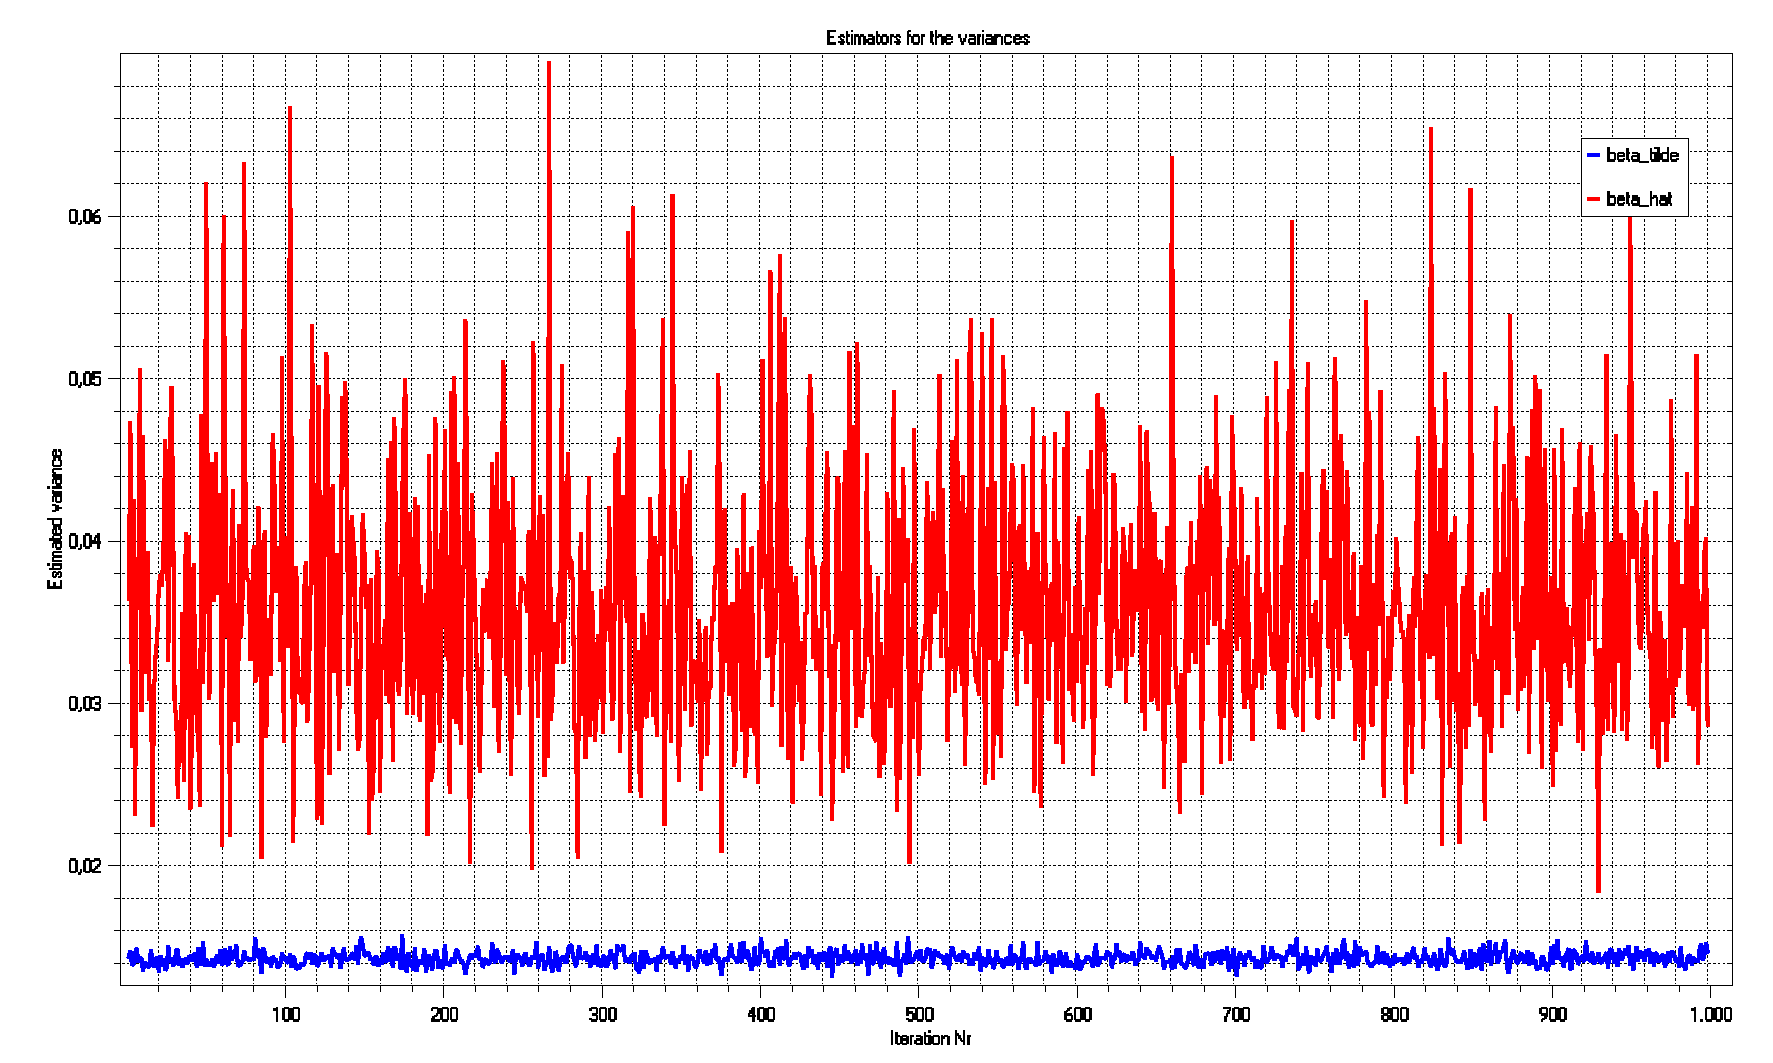
\includegraphics[height=100mm]{variance_estimators.pdf}
\caption{Variance estimations for $\hat{\beta}$ and $\tilde{\beta}$}
\label{estimated variances}
\end{figure}

\end{document}